
\chapter{Arnoldi, FOM e GMRES}
\label{chap:gmes}

Há uma unanimidade entre os pesquisadores da área de métodos iterativos para solução de sistemas lineares: não existe o melhor método para a solução de problemas com matrizes não-simétricas~\cite{NachtigalReddyEtAl1992How}. Outro ponto de vista comum é o de que, para matrizes não-normais, há muito ainda o  que se trabalhar na compreensão dos fatores que influenciam na convergência dos métodos, em especial quando se reiniciam as iterações devido ao aumento do subespaço de Krylov \cite{Meurant2024}. Ainda outro consenso, é o da necessidade de precondicionadores para acelerar os métodos de projeção em subespaços de Krylov (MPSK). Na Seção \ref{arnol_sec_arnol}, o método de Arnoldi,  um dos procedimentos seminais dos MPSK, ao lado do método de Lanczos, é discutido a partir de uma motivação para a sua construção e várias de suas propriedades são relacionadas. Nas demais seções, discutimos dois métodos paradigmáticos: o FOM e o GMRES. A literatura sobre esses métodos é vasta, estando consolidada, por exemplo, nos livros \cite{Brezinski2002Outils}, \cite{Greenbaum97Iterative}, \cite{Meurant2020Krylov} \cite{Saad03Iterative},  \cite{Vorst03Iterative}.  Ao fim deste trabalho, tocamos levemente na questão de estabilidade do GMRES quando do uso  do procedimento de Arnoldi baseado no método de reflexões de Householder ou no método de ortogonalização de Gram-Schmidt modificado,  apresentando a bibliografia necessária ao estudo deste tema. 

\section{Método de Arnoldi}\label{arnol_sec_arnol}
O nome de Arnoldi\footnote{Walter Edwin Arnoldi (1917-1995) foi um engenheiro americano que publicou sua técnica em 1951, não muito distante do aparecimento do algoritmo de Lanczos. Arnoldi graduou-se em engenharia mecânica no Stevens Institute of Technology, Hoboken, New
Jersey, em 1937 e o seu mestrado foi obtido na Harvard University em 1939. Durante sua carreira, trabalhou como engenheiro na Hamilton Standard Division da United Aircraft Corporation, aonde, com o passar do tempo, tornou-se pesquisador chefe da divisão. Aposentou-se em 1977. Apesar de sua pesquisa ter versado sobre propriedades mecânicas e aerodinâmicas de aeronaves e estruturas aeroespaciais, o nome de Arnoldi é mantido vivo graças ao seu procedimento de ortogonalização (traduzido de \cite{Meyer00Matrix}).} aparece tanto ligado à solução de problemas de autovalores quanto à solução de sistemas lineares.  Apresentaremos o método de Arnoldi \cite{Arnoldi51principle} para ortogonalizar uma base de um subespaço Krylov.
 Visando facilitar o desenvolvimento, vamos supor que o grau do polinômio mínimo  de $r_0$ em relação a $A$ é maior do que $k$.

Uma motivação interessante para o método de Arnoldi é apresentada em \cite[pág. 337]{Meurant1999Computer} e foi formulada originalmente por Kees Vuik. Queremos construir uma base ortonormal para $\mathcal{K}_k(A,r_0)$ $=\gera{r_0,Ar_0,\ldots,A^{k-1}r_0}$, tal que $\mathcal{K}_k(A,r_0)$ $=\gera{v_1,v_2,\ldots,v_{k-1},v_k}$. Seja $V=\begin{pmatrix}v_1&v_2&\ldots &v_k\end{pmatrix}$, logo $V^HV=I$. Vale, também, observar que a matriz de Krylov  associada a $\mathcal{K}_k(A,r_0)$, ${K}_k=\begin{pmatrix} r_0&Ar_0&\ldots&A^{k-1}r_0\end{pmatrix}$, goza da seguinte propriedade:
\begin{gather}
A{K}_k=\begin{pmatrix} Ar_0&A^2r_0&\ldots&A^kr_0\end{pmatrix}=\notag\\
=\begin{pmatrix} Ar_0&A^2r_0&\ldots&A^{k-1}r_0&0\end{pmatrix} +\begin{pmatrix} 0&0&\ldots&A^kr_0\end{pmatrix}=\notag\\
={K}_k\begin{pmatrix}
0 & 0 & \ldots & 0 & 0 \\
1 & 0 & \ldots & 0 & 0  \\
0 & 1& \ddots & \vdots & \vdots\\
\vdots & \vdots & \ddots & 0 & 0\\
0 & \ldots & \ldots & 1 & 0 \\
\end{pmatrix}+A^kr_0e_k^H. \label{eq_arnoldi_krylhesse}
\end{gather}
onde $e_k$ é o $k$-ésimo vetor da base canônica. Como buscamos uma base ortonormal, o método usual é o da fatoração ${K}_k=QR$, onde $Q$ é uma matriz $m\times k$, cujas colunas são vetores ortonormais, e $R$ é uma matriz não singular e triangular superior. Chamando de $H_1$ a matriz de Hessenberg que aparece em \eqref{eq_arnoldi_krylhesse}, teremos
\[AQR=QRH_1+A^kr_0e_k^H.\]
Mais algumas contas:

\begin{multline}
AQ=(QRH_1+A^kr_0e_k^H)R^{-1}\Rightarrow Q^HAQ=(RH_1+Q^HA^kr_0e_k^H)R^{-1}\Rightarrow\\
\Rightarrow Q^HAQ=R(H_1+R^{-1}Q^HA^kr_0e_k^H)R^{-1}\label{eq:vuik2},
\end{multline}
ora
\[H_2:=H_1+R^{-1}Q^HA^kr_0e_k^H=\begin{pmatrix}
    0 & 0 & \ldots & 0 & \vdots \\
     1 & 0 & \ldots & 0 & \vdots  \\
     0 & 1& \ddots & \vdots & R^{-1}Q^HA^kr_0 \\
     \vdots & \vdots & \ddots & 0 & \vdots\\
     0 & \ldots & \ldots & 1 & \vdots \\
     \end{pmatrix},\]
     é uma matriz de Hessenberg e $RH_2R^{-1}$ também o será, já que  $R$ e $R^{-1}$ são triangulares superiores. E assim, vemos que a decomposição $Q^HAQ$ é uma matriz de Hessenberg superior. E, podemos tomar para $V$ as colunas de $Q$.

%\ifthenelse{\boolean{versaocnmac}}{}
{
     Vamos desenvolver a  última  coluna de $RH_2R^{-1}$:
   
     \begin{multline*}
          RH_2R^{-1}=R(H_1+R^{-1}Q^HA^kr_0e_k^H)R^{-1}=RH_1R^{-1}+Q^HA^kr_0e_k^HR^{-1}=\\
          =RH_1R^{-1}+Q^HA^kr_0R^{-1}(k,k).
          \end{multline*}

     A última coluna do resultado é  igual a $Q^HA^kr_0R^{-1}(k,k)$. Lembrando o processo de ortogonalização de Gram-Schmidt, $R^{-1}(k,k)$ é igual a $1/\norma{\widetilde{Q}(:,k)}_2$, onde $\widetilde{Q}(:,k)$ é um vetor ortogonal aos anteriores  e ao ser normalizado resulta em ${Q}(:,k)$, ou seja, ${Q}(:,k)=\widetilde{Q}(:,k)/\norma{\widetilde{Q}(:,k)}_2$. E assim, comparando as  últimas colunas das matrizes $Q^HAQ$ e $RH_2R^{-1}$, ver \eqref{eq:vuik2}, temos
     \[
     Q^HA{Q}(:,k)=Q^HA^kr_0/\norma{\widetilde{Q}(:,k)}_2,
     \]
     ou ainda
     \[QQ^HA\widetilde{Q}(:,k)=QQ^HA^kr_0.\]
     Ou seja, as projeções ortogonais de $A\widetilde{Q}(:,k)$ e de $A^kr_0$ no subespaço de Krylov $\mathcal{K}_k(A,r_0)$ são  as mesmas. não temos ainda a resposta final, mas uma boa pista, de como gerar os subespaço de Krylov sem utilizar $A^kr_0$. Será que no processo de ortogonalização, ao substituirmos  o vetor $A^kr_0$ pelo vetor $A\widetilde{Q}(:,k)$, estaremos gerando bases para o mesmo subespaço de Krylov $\mathcal{K}_k(A,r_0)$? Quais as condições sobre os vetores $A^kr_0$ e $A\widetilde{Q}(:,k)$ para que os subespaços gerados sejam os mesmos? A resposta positiva é o método de Arnoldi que está descrito nos Algoritmos \ref{algor_arnoldigs} e \ref{algor_arnoldigsm}.
}
     \begin{algor}[htb]
\caption{ Método  de Arnoldi $(A,\;r_0,\;k)$ - alternativa com Gram-Schmidt clássico.} \label{algor_arnoldigs}

{%\footnotesize
\begin{enumerate}
\renewcommand{\labelenumi}{\theenumi:}
\setlength{\itemsep}{.01cm}
\item $V(:,1)=r_0/\norma{r_0}$
\item para $j=1:k$
\item~~~$w=AV(:,j)$
\item~~~$H(1:j,j)=V(:,1:j)^Hw$
\item~~~$w=(I-V(:,1:j)V(:,1:j)^H)w$
\item~~~$H(j+1,j)=\norma{w}_2$
\item~~~$V(:,j+1)=w/H(j+1,j)$
\item fim-para
\renewcommand{\labelenumi}{\theenumi.}
\end{enumerate}
}
\end{algor}
O Algoritmo \ref{algor_arnoldigs} usa o processo de ortogonalização de Gram-Schmidt clássico, onde todos os escalares  utilizados para multiplicar os elementos da base já  existente são  calculados usando o mesmo valor de $w=AV(:,j)$. Esse procedimento é numericamente instável, e por razões de estabilidade uma versão  modificada é utilizada \cite{Stewart1973Introduction}\footnote{Para ver exemplo de instabilidade consultar, entre outros, \cite[exemplo 5.5.5, pág. 316]{Meyer00Matrix}.}, ver Algoritmo \ref{algor_arnoldigsm}.
     \begin{algor}[htb]
\caption{ Método  de Arnoldi $(A,\;r_0,\;k)$  - alternativa com  Gram-Schmidt modificado.}\label{algor_arnoldigsm}

  {%\footnotesize
\begin{enumerate}
\renewcommand{\labelenumi}{\theenumi:}
\setlength{\itemsep}{.01cm}
\item $V(:,1)=r_0/\norma{r_0}_2$
\item para $j=1:k$
\item\label{algor_arnoldigsm_it_wav}~~~$w=AV(:,j)$
\item~~~para $i=1:j$
\item~~~~~~$H(i,j)=(V(:,i),w)$
\item~~~~~~$w=w-H(i,j)V(:,i)$
\item~~~fim-para
\item\label{algor_arnoldigsm_hj1j}~~~$H(j+1,j)=\norma{w}_2$
\item\label{algor_arnoldigsm_vj1}~~~$V(:,j+1)=w/H(j+1,j)$
\item fim-para
\renewcommand{\labelenumi}{\theenumi.}
\end{enumerate}
}
\end{algor}
\begin{obs}\label{obs_arnoldiruptura}
Em ambas as versões do algoritmo de Arnoldi ainda não há um teste  sobre  $H(j+1,j)$ ser numericamente zero (ou seja, menor que uma constante arbitrada). Esse fato, denominado de \textbf{ruptura} do algoritmo, ocorre quando o novo vetor pertence em precisão finita ao mesmo subespaço dos vetores  gerados  até  aquele momento. Ou seja, quando $\mathcal{K}_k(A,r_0)\supset A\mathcal{K}_k(A,r_0)$ ou, ainda, $\mathcal{K}_k(A,r_0)= \mathcal{K}_{k+1}(A,r_0)$. Em uma real implementação computacional é necessária a inclusão  de um teste de ruptura.
\end{obs}
\begin{obs}\label{obs_mgsgsdif}
Em \cite[pág. 279]{Stewart98Matrix}, o autor é bastante enfático quanto a inadequação do nome Gram-Schmidt modificado, uma vez que ele considera ser outro método com outras propriedades apesar da semelhança entre os algoritmos, para maiores detalhes ver a obra citada.
\end{obs}
Sejam $V_k\in\mathbb{C}^{m\times k}$, a matriz cujas colunas são  os vetores $V(:,j)$, e $H_k\in\mathbb{C}^{k\times k}$, a matriz Hessenberg superior, formadas no procedimento de Arnoldi  até  a $k$-ésima iteração do Algoritmo \ref{algor_arnoldigsm} antes de executarmos os passos \ref{algor_arnoldigsm_hj1j}: e \ref{algor_arnoldigsm_vj1}:. O algoritmo completo, contadas as $k$ iterações, terá uma representação matricial,  até  esse momento, dada por
\begin{equation}\label{arnol_prop_avk-vkhwekh}
AV_k-V_kH_k=we_k^H,
\end{equation}
onde $e_k$ é o $k$-ésimo vetor da base canônica. Ao incorporarmos os passos  \ref{algor_arnoldigsm_hj1j}: e \ref{algor_arnoldigsm_vj1}:, passamos a ter:

\begin{gather}
AV_k-V_kH_k=H(k+1,k)V(:,k+1)e_k^H \Rightarrow \notag\\ \Rightarrow AV_k=V_kH_k+H(k+1,k)V(:,k+1)e_k^H\label{arnol_prop_soma}.
\end{gather}
Temos aqui uma multiplicação entre matrizes representada por um produto externo e podemos escrevê-la de forma mais compacta como:
\begin{equation}\label{arnol_prop_comple}
AV_k=V_{k+1}\overline{H}_k,
\end{equation}
onde $V_{k+1}\in\mathbb{C}^{m\times (k+1)}$ e $\overline{H}_k\in\mathbb{C}^{(k+1)\times k}$.
Há, ainda, uma relação simples a ser extraída:
\begin{equation}\label{arnol_prop_hk}
V_k^HAV_k={H}_k.
\end{equation}



 As fórmulas \eqref{arnol_prop_soma}, \eqref{arnol_prop_comple} e \eqref{arnol_prop_hk} resumem algumas das propriedades do método de Arnoldi que usaremos adiante.

 \begin{obs}\label{arnol_obs_vkavk}
 Vale observar que a fórmula \eqref{arnol_prop_hk} nos lembra  a decomposição de Schur (só que na decomposição de Schur, $V_k$ é, necessariamente, quadrada), ver ~\cite[pág. 79]{HornJohnson1985}. E, motivados por essa observação, podemos utilizar autovalores relacionados à matriz ${H}_k$ visando aumentar a velocidade de convergência dos  métodos de Krylov baseados no procedimento de Arnoldi.
 \end{obs}

\section{Ortogonalização Completa - FOM}\label{arnol_sec_fom}

Para resolver $Ax=b$, o método da \textbf{ortogonalização completa}~\cite{Saad1981Krylov}, \cite{Saad03Iterative} é um MPSK com as seguintes características:  partindo de um valor inicial $x_0$, tem-se o  resíduo inicial, $r_0=b-Ax_0$. $\mathcal{K}_k$ será o subespaço de Krylov $\mathcal{K}_k(A,r_0)$. A cada nova iteração, calcula-se $x_k$  impondo as condições: $(x_k-x_0)\in \mathcal{K}_k(A,r_0)$ e o  resíduo $r_k=b-Ax_k$ deve ser ortogonal à $\mathcal{L}_k=\mathcal{K}_k(A,r_0)$. Nesse caso, o espaço de restrições será $\mathcal{L}_k=\mathcal{K}_k$ e $r_k\perp \mathcal{K}_k(A,r_0)$. Uma representação gráfica simplificada desse fato pode ser vista na figura \ref{fig_kryakrybfom}.

\begin{figure}[htb]
  % Requires \usepackage{graphicx}
  \epsfig{file=Figures/arnol_fom.eps, width=\linewidth}
  \caption{Representação esquemática da condição de ortogonalidade do  resíduo do FOM.}\label{fig_kryakrybfom}
\end{figure}

Uma representação resumida da estrutura de uma iteração do FOM é apresentada no Algoritmo \ref{algor_fomesquema}.
     \begin{algor}[htb]
\caption{Ortogonalização completa $(A,\;x_0)$ - resumo de uma iteração}\label{algor_fomesquema}
{%\footnotesize
\begin{enumerate}
\renewcommand{\labelenumi}{\theenumi:}
\setlength{\itemsep}{.01cm}
\item\label{algor_fomesquema_arnoldi} adicionar um vetor a uma base ortonormal para o subespaço de Krylov $\mathcal{K}_j(A,r_0)$,
\item\label{algor_fomesquema_xjrj} calcular $x_j$ tal que $x_j-x_0\in \mathcal{K}_j(A,r_0)$ e que $r_j\perp \mathcal{K}_j(A,r_0)$.
\renewcommand{\labelenumi}{\theenumi.}
\end{enumerate}
}
\end{algor}
O primeiro passo do Algoritmo \ref{algor_fomesquema} será feito pelo método de Arnoldi. No segundo passo, as condições dadas nos permitem detalhar as operações matriciais necessárias. Seja $V_j$ uma base ortonormal para $\mathcal{K}_j(A,r_0)$, então temos que para algum $y_j\in\mathbb{C}^j$, $x_j-x_0=V_jy_j$, o que atende à primeira condição. Quanto ao  resíduo, ele tem que ser ortogonal ao mesmo espaço, ou seja $r_j^HV_j=0$ ou $V_j^Hr_j=0$, mas
\begin{multline*}
r_j=b-Ax_j=b-A(x_0+V_jy_j)=r_0-AV_jy_j\Rightarrow V_j^H(r_0-AV_jy_j)=0\Rightarrow \\ \Rightarrow V_j^HAV_jy_j=V_j^Hr_0 \Rightarrow H_jy_j=V_j^Hr_0.
\end{multline*}
Como essa base é ortonormal e o primeiro vetor da base é, exatamente, $r_0/\norma{r_0}_2$, então $V_j^Hr_0=\big((r_0/\norma{r_0}_2)^Hr_0,0,\ldots,0\big)$. Logo, temos que resolver o sistema
\[
H_jy_j=\norma{r_0}_2 e_1,
\]
onde $e_1$ é o primeiro vetor da base canônica de $\mathbb{C}^j$. Para que esse sistema tenha solução única é necessáro e suficiente que $H_j$ seja uma matriz não singular. Essa condição não será sempre garantida e a singularidade de $H_j$ pode ocorrer em duas situações distintas. No primeiro caso, será uma ruptura benéfica do algoritmo:
\[
H_jy_j=0\Rightarrow V_j^HAV_jy_j=0\Rightarrow V_j^HA\sum_{i=1}^j\alpha_iv_i=0,
\]
como as colunas de $V_j$ geram uma base para   $\mathcal{K}_j(A,r_0)$ temos ainda que
\[
V_j^HA\sum_{i=1}^j\alpha_iv_i=0\Rightarrow V_j^HA\sum_{i=1}^j\alpha_i\bigg(\sum_{k=1}^j\beta_k A^{k-1}r_0\bigg)=0,
\]
nesse caso, vamos considerar que $AV_jy_j=0$
\[
A\sum_{i=1}^j\alpha_i\bigg(\sum_{k=1}^j\beta_k A^{k-1}r_0\bigg)=0\Rightarrow \sum_{i=1}^j \gamma_i A^ir_0=0,
\]
ou seja chegamos ao polinômio mínimo de $r_0$ em relação a $A$ e temos a solução exata.

Mas outra situação também pode ocorrer, nesse caso $z_j:=AV_jy_j\neq 0$ e $V_j^Hz_j=0$, ou seja, existe um vetor não-nulo em $A\mathcal{K}_j(A,r_0)$ que é ortogonal a $\mathcal{K}_j(A,r_0)$, também nesse caso a matriz $H_j$ será singular e haverá uma ruptura do FOM, sem ser benéfica.

O próximo resultado mostra como o cálculo do  resíduo é simples para o FOM.

\begin{teore}
O  resíduo da $j$-ésima iteração do FOM é dado por

\[
r_j=-\overline{H}_j(j+1,j)V_{j+1}(:,(j+1)) e_j^T y_j \quad\text{e}\quad \norma{r_j}_2=\overline{H}_j(j+1,j)|e_j^T y_j|.
\]


\end{teore}
\dem
\begin{eqnarray*}
r_j&=&b-Ax_j=b-Ax_0-AV_jy_j=r_0-V_{j+1}\overline{H}_jy_j=\\
&=&r_0-(V_jH_j+\overline{H}_j(j+1,j)V_{j+1}(:,(j+1))e_j^T)y_j=\\
&=&\beta V_j e_1-(V_jH_j+\overline{H}_j(j+1,j)V_{j+1}(:,(j+1))e_j^T)y_j=\\
&=&V_j(\beta  e_1-H_jy_j)-\overline{H}_j(j+1,j)V_{j+1}(:,(j+1))e_j^T y_j=\\
&=&-\overline{H}_j(j+1,j)V_{j+1}(:,(j+1))e_j^T y_j.\\
\end{eqnarray*}
Como $\overline{H}_j(j+1,j)e_j^T y_j$ é um escalar e $\norma{V_{j+1}(:,(j+1))}_2=1$, temos os resultados.
\fim

\markboth{Arnoldi}{ Resíduo Minimal Generalizado - GMRES}

\section{Resíduo Minimal Generalizado - GMRES}\label{arnol_sec_gmres}
O método de \textbf{ resíduo minimal generalizado (GMRES)}~\cite{SaadSchultz86GMRES} é um MPSK com as seguintes características. Para resolvermos $Ax=b$, partimos de um valor inicial $x_0$ e  calculamos o  resíduo inicial, $r_0=b-Ax_0$. $\mathcal{K}_k$ será o subespaço de Krylov $\mathcal{K}_k(A,r_0)$, ou seja, $(x_k-x_0)\in \mathcal{K}_k(A,r_0)$, e o espaço de restrições será $\mathcal{L}_k=A\mathcal{K}_k(A,r_0)$ e, assim, o  resíduo $r_k$ é ortogonal a $A\mathcal{K}_k(A,r_0)$, $r_k\perp A\mathcal{K}_k(A,r_0)$. Com isso, o GMRES assegura que o  resíduo, a cada iteração, não aumentará, no pior caso o  resíduo  das novas iterações será igual ao(s) da(s) anterior(es). Como a cada passo o espaço de busca está aumentando, mesmo depois de alguma \textbf{estagnação}, o método encontrará um ponto melhor. Uma representação gráfica simplificada desse fato pode ser vista na figura \ref{fig_kryakrybgmres}.

\begin{figure}[htb]
  % Requires \usepackage{graphicx}
  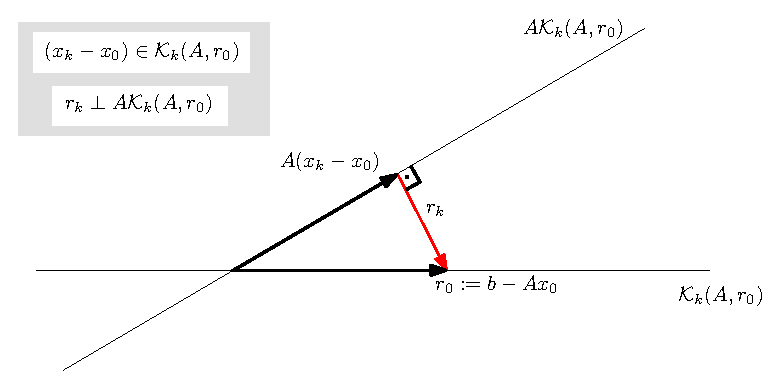
\epsfig{file=Figures/arnol_gmres.eps, width=\linewidth}
  \caption{Representação esquemática da condição de ortogonalidade do  resíduo do GMRES.}\label{fig_kryakrybgmres}
\end{figure}


     \begin{algor}[htb]
\caption{GMRES $(A,\;x_0)$ - resumo de uma iteração}\label{algor_gmresesquema}
{%\footnotesize
\begin{enumerate}
\renewcommand{\labelenumi}{\theenumi:}
\setlength{\itemsep}{.01cm}
\item\label{algor_gmresesquema_arnoldi} adicionar um vetor a uma base ortonormal para o subespaço de Krylov $\mathcal{K}_j(A,r_0)$,
\item\label{algor_gmresesquema_xjrj} calcular $x_j$ tal que $x_j-x_0\in \mathcal{K}_j(A,r_0)$ e que $r_j\perp A\mathcal{K}_j(A,r_0)$.
\renewcommand{\labelenumi}{\theenumi.}
\end{enumerate}
}
\end{algor}

Uma representação resumida da estrutura de uma  iteração do GMRES é apresentada no Algoritmo \ref{algor_gmresesquema}, aonde o passo \ref{algor_gmresesquema_arnoldi}: será realizado através do método de Arnoldi e no passo \ref{algor_gmresesquema_xjrj}: haverá a solução de um problema de quadrados mínimos através de uma fatoração $QR$ adequada.
Vejamos alguns dos detalhes desse processo:
\[
r_k=b-Ax_k=b-A(x_0+c_k)=r_0-Ac_k, \quad c_k\in\mathcal{K}_k(A,r_0);
\]
sejam $V_{k+1}$ uma matriz cujas colunas formam uma base ortonormal  para $\mathcal{K}_{k+1}(A,r_0)$ e $V_k$ uma matriz cujas colunas formam uma base ortonormal  para $\mathcal{K}_k(A,r_0)$, então $c_k=V_k y_k$, $y_k\in\mathbb{C}^k$, e podemos continuar o desenvolvimento acima,  lembrando-nos de uma das relações de Arnoldi, $AV_k=V_{k+1}\overline{H}_k$:
\[
r_k=r_0-Ac_k=r_0-AV_ky_k=r_0-V_{k+1}\overline{H}_ky_k.
\]
Na construção da base ortonormal consideramos $v_1=r_0/\norma{r_0}_2$, logo
\[
r_0-V_{k+1}\overline{H}_ky_k=\norma{r_0}_2v_1-V_{k+1}\overline{H}_ky_k=\norma{r_0}_2V_{k+1}e_1-V_{k+1}\overline{H}_ky_k
\]
temos, então
\[
r_k=V_{k+1}(\norma{r_0}_2e_1-\overline{H}_ky_k),
\]
 mas $\norma{V_{k+1}}_2=1$, uma vez que as suas colunas são  vetores ortonormais, logo o problema de quadrados mínimos que temos que resolver é
\begin{equation}\label{eq_gmresquadmin}
\norma{r_k}_2=\underset{y_k\in \mathbb{C}^k}{\min}\norma{\norma{r_0}_2e_1-\overline{H}_ky_k}_2.
\end{equation}

Desenvolvendo \eqref{eq_gmresquadmin}. Podemos construir o produto matricial \begin{equation}\label{eq_gmresquadminnovoproduto}
\norma{\begin{pmatrix}\overline{H}_k & \norma{r_0}_2e_1\\\end{pmatrix}\begin{pmatrix}
                                                                  y_k \\
                                                                  -1 \\
                                                                \end{pmatrix}}_2.
\end{equation}
Fazendo a fatoração $QR$ de \[
\begin{pmatrix}\overline{H}_k & \norma{r_0}_2e_1\\\end{pmatrix}=Q_{k+1}R_{k+1}= Q_{k+1} \begin{pmatrix}R_k & \zeta\\0 & s\end{pmatrix}.
       \]
E \eqref{eq_gmresquadminnovoproduto} pode ser escrita como:
\begin{equation}\label{eq_gmresquadminnovoprodutosemqk1}
\norma{ Q_{k+1}\begin{pmatrix}R_k & \zeta\\0 & s\end{pmatrix} \begin{pmatrix}y_k \\ -1 \\  \end{pmatrix}}_2=\norma{ \begin{pmatrix}R_k & \zeta\\0 & s\end{pmatrix} \begin{pmatrix}y_k \\ -1 \\  \end{pmatrix}}_2.
\end{equation}
Logo a expressão  \eqref{eq_gmresquadmin}, transforma-se em
\begin{equation}\label{eq_gmresquadminnovamin}
\norma{r_k}_2=\underset{y_k\in \mathbb{C}^k}{\min}\norma{\begin{pmatrix}R_k y_k-\zeta \\ s  \end{pmatrix}}_2= |s|.
\end{equation}
O que fornece uma forma simples\label{arnol_calcuresid} de se calcular a norma do  resíduo, pelo menos em aritmética exata (ou infinita). Essa informação será útil tanto para detectar a convergência do método como para observar algum processo de estagnação\footnote{No entanto \label{arnol_calcuresidprob} um alerta deve ser feito aqui, pois esse cálculo, quando feito em aritmética  finita, pode levar a  erro, uma vez que a igualdade pode não estar garantida, para maiores esclarecimentos desse fenômeno consultar \cite[pág. 90]{Chaitin-ChatelinFraysse1996Lectures}.}.

Relembrando a observação \ref{obs_arnoldiruptura}, haverá um momento em que $H(k+1,k)=0$, isso significa que  o novo vetor calculado pertence ao espaço de Krylov anterior ou seja $w\in\mathcal{K}_k(A,r_0)$, confira o Algoritmo \ref{algor_arnoldigsm}. 

A implementação do GMRES baseia-se na utilização de rotações de Givens para resolver o problema de quadrados mínimos. Como $\overline{H}_k$ é uma matriz de Hessenberg superior, as rotações são  utilizadas para anular todos os valores que se encontram exatamente abaixo da diagonal principal. As rotações atuam apenas em uma entrada por vez, o trabalho feito anteriormente é aproveitado, sendo uma alternativa atraente por sua economia e estabilidade.

No artigo inicial sobre o GMRES \cite{SaadSchultz86GMRES} foram apresentados resultados de convergência do método para matrizes normais. No entanto, segundo \cite{Vorst03Iterative}, o principal resultado sobre a convergência do GMRES para uma matriz qualquer é, no mínimo, intrigante e foi apresentado em \cite{GreenbaumPtakEtAl96Any}, em 1996.
\begin{teore}[Convergência do GMRES]\label{teo_gmresconverg}
Dada uma  sequência não crescente de reais positivos $f_0\ge f_1\ge\ldots \ge f_{m+1}$ e um conjunto de complexos não nulos $\lambda_1,\lambda_1,\ldots,\lambda_m$, então existe uma matriz $A$ com autovalores $\lambda_j$ e com lado direito $b=f_0e_1$ tal que os  resíduos $r_k$ do GMRES calculados na solução de $Ax=b$, com $x_0=0$, satisfazem $\norma{r_k}_2=f_k$, para $k=0:(n-1)$.
\end{teore}
\begin{obs}\label{obs_gmresconv}
O teorema \ref{teo_gmresconverg} nos informa que para uma matriz qualquer apenas os autovalores não são  suficientes para caracterizar o comportamento da convergência do GMRES. No entanto, para matrizes normais, os autovalores são  suficientes. também para matrizes bem condicionadas, mesmo que não normais, os autovalores dão informação sobre o a convergência do  método.
\end{obs}
\begin{obs}\label{obs_gmresconvcontraponto}
O outro lado da moeda do teorema \ref{teo_gmresconverg} é que, na prática, ele não influencia o uso ou não do GMRES, apenas dá uma informação sobre casos possíveis e não sobre casos que sempre ocorrerão. Um outro aspecto é que o GMRES tem, em muitos casos importantes, uma convergência lenta, necessitando de precondicionadores para funcionar em um número de iterações aceitável, nesse caso a informação fornecida pelo teorema não tem grande aplicação.
\end{obs}

 A discussão  sobre as ferramentas matemáticas para caracterização da convergência do GMRES, e dos demais  métodos de Krylov para matrizes não-normais, é uma área de estudo importante e que contém vários problemas em aberto, ver por exemplo \cite{Embree1999How},  \cite{PaigeParlettEtAl95Approximate}, \cite{SimonciniSzyld2007Recent}, \cite{Zemke2003Krylov}.

 Um comentário necessáro  é sobre a estabilidade do método GMRES. Há dois resultados em \cite{PaigeRozloznikEtAl2006MODIFIED} e \cite{Rozloznik1997Numerical} onde são  caracterizadas a estabilidade em relação ao erro inverso das implementações do GMRES usando as reflexões de Householder e o método modificado de Gram-Schmidt no processo de Arnoldi. Esses resultados asseguram que pequenas modificações nos dados tratados não irão acarretar grandes problemas na solução do problema, uma vez que se estará  resolvendo exatamente um problema próximo. Ou seja a dificuldade será  intrínseca ao prôprio sistema que está sendo resolvido e não devida ao algoritmo utilizado. Trata-se de uma leitura  técnica e importante para os pesquisadores da área.



A versão  utilizada na prática para o GMRES é a \textbf{com recomeço}. Com o avanço do número de iterações do GMRES, o armazenamento dos vetores necessáros e o tamanho dos problemas de quadrados mínimos a serem resolvidos começam a inviabilizar a aplicação do  método. Há várias alternativas: a escolha de um subconjunto reduzido dos vetores já  calculados  e o recomeço após de um número fixado de iterações (versões com recomeço). A versão  com recomeço padrão simplesmente testa a convergência depois de um número fixo de iterações  e, caso não se tenha atingido a cota desejada, mantêm-se apenas a  última  aproximação, descartando-se todos os demais vetores,  e usa-se esse aproximação como valor inicial para calcular um novo  resíduo inicial e  começar uma nova aplicação do GMRES\footnote{Cada ciclo completo de recomeço é denominado \textbf{ciclo} do GMRES.}, ver análises em \cite{Morgan95Restarted}, \cite{Simoncini00Convergence} e \cite{Trefethen1990Algorithms}. A vantagem dessa alternativa é que como cada iteração garante o não aumento da norma euclidiana do  resíduo, com o uso dessa solução, garante-se que estaremos partindo de um ponto, possivelmente melhor do que a primeira aproximação $x_0$. Apesar de  drástica, essa alternativa é das mais usadas na prática. A bem da verdade, a alternativa com recomeço é um método de Krylov apenas durante cada ciclo do GMRES, uma vez que a cada recomeço um novo subespaço de Krylov é construído, ou seja o método completo não fica dentro de um mesmo subespaço de Krylov que aumenta a cada ciclo completo.

Há dezenas de variantes do  GMRES que foram desenvolvidas nos últimos 20 anos, ver por exemplo \cite{SaadVorst00Iterative,SimonciniSzyld2007Recent,Zou2023}.

